

\tikzset{every picture/.style={line width=0.75pt}} %set default line width to 0.75pt        

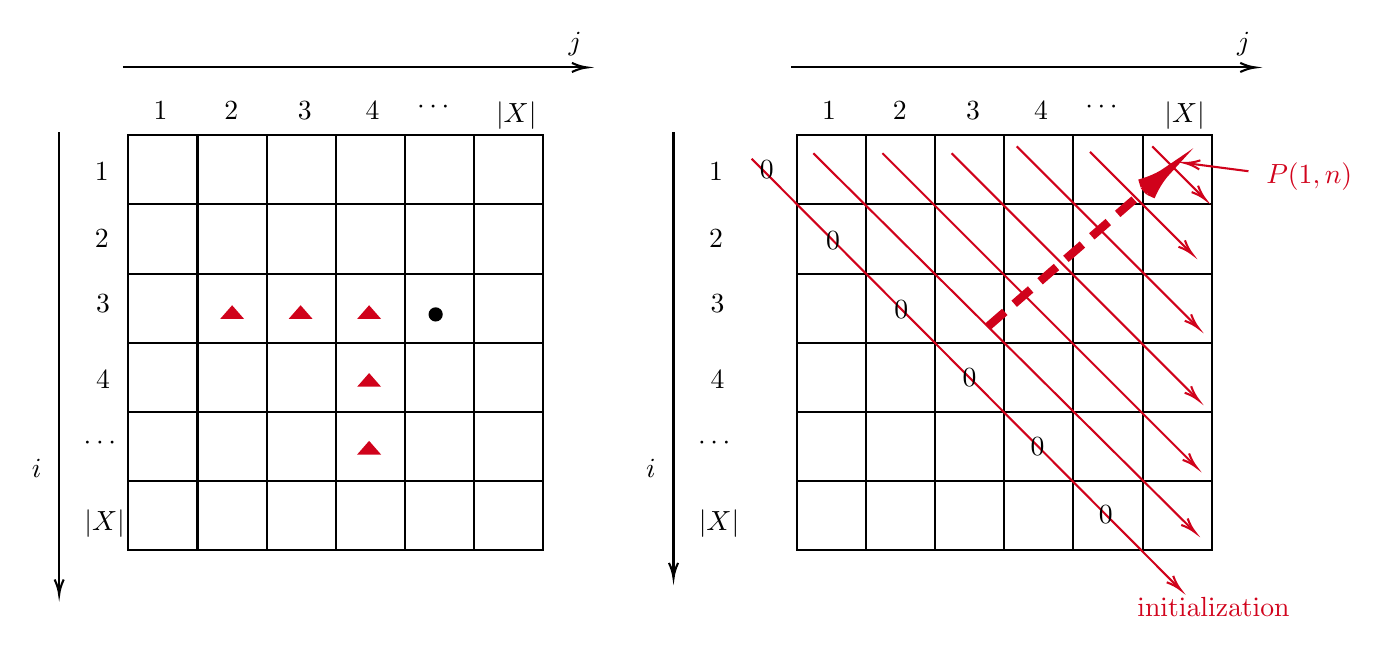
\begin{tikzpicture}[x=0.5pt,y=0.5pt,yscale=-1,xscale=1]
%uncomment if require: \path (0,447); %set diagram left start at 0, and has height of 447

%Shape: Grid [id:dp9095284515127875] 
\draw  [draw opacity=0] (87,90) -- (387,90) -- (387,390) -- (87,390) -- cycle ; \draw   (137,90) -- (137,390)(187,90) -- (187,390)(237,90) -- (237,390)(287,90) -- (287,390)(337,90) -- (337,390) ; \draw   (87,140) -- (387,140)(87,190) -- (387,190)(87,240) -- (387,240)(87,290) -- (387,290)(87,340) -- (387,340) ; \draw   (87,90) -- (387,90) -- (387,390) -- (87,390) -- cycle ;
%Straight Lines [id:da5347307434268296] 
\draw    (37,88) -- (37,420) ;
\draw [shift={(37,422)}, rotate = 270] [color={rgb, 255:red, 0; green, 0; blue, 0 }  ][line width=0.75]    (10.93,-3.29) .. controls (6.95,-1.4) and (3.31,-0.3) .. (0,0) .. controls (3.31,0.3) and (6.95,1.4) .. (10.93,3.29)   ;
%Straight Lines [id:da4989887299865372] 
\draw    (83,41) -- (416.5,41) ;
\draw [shift={(418.5,41)}, rotate = 180] [color={rgb, 255:red, 0; green, 0; blue, 0 }  ][line width=0.75]    (10.93,-3.29) .. controls (6.95,-1.4) and (3.31,-0.3) .. (0,0) .. controls (3.31,0.3) and (6.95,1.4) .. (10.93,3.29)   ;
%Flowchart: Connector [id:dp07878936208838816] 
\draw  [fill={rgb, 255:red, 0; green, 0; blue, 0 }  ,fill opacity=1 ] (305,217.9) .. controls (305.87,215.65) and (308.4,214.52) .. (310.66,215.39) .. controls (312.91,216.26) and (314.04,218.79) .. (313.17,221.05) .. controls (312.3,223.3) and (309.77,224.43) .. (307.51,223.56) .. controls (305.26,222.69) and (304.13,220.16) .. (305,217.9) -- cycle ;
%Shape: Triangle [id:dp6109876057002935] 
\draw  [color={rgb, 255:red, 208; green, 2; blue, 27 }  ,draw opacity=1 ][fill={rgb, 255:red, 208; green, 2; blue, 27 }  ,fill opacity=1 ] (261,214) -- (268,222) -- (254,222) -- cycle ;
%Shape: Triangle [id:dp003677095504452388] 
\draw  [color={rgb, 255:red, 208; green, 2; blue, 27 }  ,draw opacity=1 ][fill={rgb, 255:red, 208; green, 2; blue, 27 }  ,fill opacity=1 ] (211.5,214) -- (218.5,222) -- (204.5,222) -- cycle ;
%Shape: Triangle [id:dp543232883301439] 
\draw  [color={rgb, 255:red, 208; green, 2; blue, 27 }  ,draw opacity=1 ][fill={rgb, 255:red, 208; green, 2; blue, 27 }  ,fill opacity=1 ] (162,214) -- (169,222) -- (155,222) -- cycle ;
%Shape: Triangle [id:dp29900180690969524] 
\draw  [color={rgb, 255:red, 208; green, 2; blue, 27 }  ,draw opacity=1 ][fill={rgb, 255:red, 208; green, 2; blue, 27 }  ,fill opacity=1 ] (261,263) -- (268,271) -- (254,271) -- cycle ;
%Shape: Triangle [id:dp5517868734647194] 
\draw  [color={rgb, 255:red, 208; green, 2; blue, 27 }  ,draw opacity=1 ][fill={rgb, 255:red, 208; green, 2; blue, 27 }  ,fill opacity=1 ] (261,312) -- (268,320) -- (254,320) -- cycle ;
%Shape: Grid [id:dp8676217076414684] 
\draw  [draw opacity=0] (570,90) -- (870,90) -- (870,390) -- (570,390) -- cycle ; \draw   (620,90) -- (620,390)(670,90) -- (670,390)(720,90) -- (720,390)(770,90) -- (770,390)(820,90) -- (820,390) ; \draw   (570,140) -- (870,140)(570,190) -- (870,190)(570,240) -- (870,240)(570,290) -- (870,290)(570,340) -- (870,340) ; \draw   (570,90) -- (870,90) -- (870,390) -- (570,390) -- cycle ;
%Straight Lines [id:da23917339503157053] 
\draw    (481,88) -- (481,408) ;
\draw [shift={(481,410)}, rotate = 270] [color={rgb, 255:red, 0; green, 0; blue, 0 }  ][line width=0.75]    (10.93,-3.29) .. controls (6.95,-1.4) and (3.31,-0.3) .. (0,0) .. controls (3.31,0.3) and (6.95,1.4) .. (10.93,3.29)   ;
%Straight Lines [id:da1200250503088851] 
\draw    (566,41) -- (899.5,41) ;
\draw [shift={(901.5,41)}, rotate = 180] [color={rgb, 255:red, 0; green, 0; blue, 0 }  ][line width=0.75]    (10.93,-3.29) .. controls (6.95,-1.4) and (3.31,-0.3) .. (0,0) .. controls (3.31,0.3) and (6.95,1.4) .. (10.93,3.29)   ;
%Straight Lines [id:da5849775638339646] 
\draw [color={rgb, 255:red, 208; green, 2; blue, 27 }  ,draw opacity=1 ]   (896.5,116) -- (852.48,110.26) ;
\draw [shift={(850.5,110)}, rotate = 367.43] [color={rgb, 255:red, 208; green, 2; blue, 27 }  ,draw opacity=1 ][line width=0.75]    (10.93,-3.29) .. controls (6.95,-1.4) and (3.31,-0.3) .. (0,0) .. controls (3.31,0.3) and (6.95,1.4) .. (10.93,3.29)   ;
%Straight Lines [id:da7158674315801672] 
\draw [color={rgb, 255:red, 208; green, 2; blue, 27 }  ,draw opacity=1 ]   (537.5,107) -- (846.09,417.08) ;
\draw [shift={(847.5,418.5)}, rotate = 225.14] [color={rgb, 255:red, 208; green, 2; blue, 27 }  ,draw opacity=1 ][line width=0.75]    (10.93,-3.29) .. controls (6.95,-1.4) and (3.31,-0.3) .. (0,0) .. controls (3.31,0.3) and (6.95,1.4) .. (10.93,3.29)   ;
%Straight Lines [id:da06318163354731099] 
\draw [color={rgb, 255:red, 208; green, 2; blue, 27 }  ,draw opacity=1 ]   (582,103) -- (856.58,375.59) ;
\draw [shift={(858,377)}, rotate = 224.79] [color={rgb, 255:red, 208; green, 2; blue, 27 }  ,draw opacity=1 ][line width=0.75]    (10.93,-3.29) .. controls (6.95,-1.4) and (3.31,-0.3) .. (0,0) .. controls (3.31,0.3) and (6.95,1.4) .. (10.93,3.29)   ;
%Straight Lines [id:da7422545951430948] 
\draw [color={rgb, 255:red, 208; green, 2; blue, 27 }  ,draw opacity=1 ]   (632,103) -- (857.59,328.59) ;
\draw [shift={(859,330)}, rotate = 225] [color={rgb, 255:red, 208; green, 2; blue, 27 }  ,draw opacity=1 ][line width=0.75]    (10.93,-3.29) .. controls (6.95,-1.4) and (3.31,-0.3) .. (0,0) .. controls (3.31,0.3) and (6.95,1.4) .. (10.93,3.29)   ;
%Straight Lines [id:da6389984033381221] 
\draw [color={rgb, 255:red, 208; green, 2; blue, 27 }  ,draw opacity=1 ]   (682,103) -- (859.09,280.09) ;
\draw [shift={(860.5,281.5)}, rotate = 225] [color={rgb, 255:red, 208; green, 2; blue, 27 }  ,draw opacity=1 ][line width=0.75]    (10.93,-3.29) .. controls (6.95,-1.4) and (3.31,-0.3) .. (0,0) .. controls (3.31,0.3) and (6.95,1.4) .. (10.93,3.29)   ;
%Straight Lines [id:da7613617756284687] 
\draw [color={rgb, 255:red, 208; green, 2; blue, 27 }  ,draw opacity=1 ]   (729,98) -- (859.09,228.09) ;
\draw [shift={(860.5,229.5)}, rotate = 225] [color={rgb, 255:red, 208; green, 2; blue, 27 }  ,draw opacity=1 ][line width=0.75]    (10.93,-3.29) .. controls (6.95,-1.4) and (3.31,-0.3) .. (0,0) .. controls (3.31,0.3) and (6.95,1.4) .. (10.93,3.29)   ;
%Straight Lines [id:da7035765059521567] 
\draw [color={rgb, 255:red, 208; green, 2; blue, 27 }  ,draw opacity=1 ]   (782,102) -- (854.59,174.59) ;
\draw [shift={(856,176)}, rotate = 225] [color={rgb, 255:red, 208; green, 2; blue, 27 }  ,draw opacity=1 ][line width=0.75]    (10.93,-3.29) .. controls (6.95,-1.4) and (3.31,-0.3) .. (0,0) .. controls (3.31,0.3) and (6.95,1.4) .. (10.93,3.29)   ;
%Straight Lines [id:da156242521236438] 
\draw [color={rgb, 255:red, 208; green, 2; blue, 27 }  ,draw opacity=1 ]   (827,98) -- (864.09,135.09) ;
\draw [shift={(865.5,136.5)}, rotate = 225] [color={rgb, 255:red, 208; green, 2; blue, 27 }  ,draw opacity=1 ][line width=0.75]    (10.93,-3.29) .. controls (6.95,-1.4) and (3.31,-0.3) .. (0,0) .. controls (3.31,0.3) and (6.95,1.4) .. (10.93,3.29)   ;
%Straight Lines [id:da421849353700268] 
\draw [color={rgb, 255:red, 208; green, 2; blue, 27 }  ,draw opacity=1 ][line width=3]  [dash pattern={on 7.88pt off 4.5pt}]  (708.5,228) -- (833.72,119.28) ;
\draw [shift={(837.5,116)}, rotate = 499.03] [color={rgb, 255:red, 208; green, 2; blue, 27 }  ,draw opacity=1 ][line width=3]    (20.77,-6.25) .. controls (13.2,-2.65) and (6.28,-0.57) .. (0,0) .. controls (6.28,0.57) and (13.2,2.66) .. (20.77,6.25)   ;

% Text Node
\draw (68,103) node [anchor=north west][inner sep=0.75pt]   [align=left] {$ $};
% Text Node
\draw (60.5,107.38) node [anchor=north west][inner sep=0.75pt]   [align=left] {$\displaystyle 1$};
% Text Node
\draw (52.5,306.14) node [anchor=north west][inner sep=0.75pt]   [align=left] {$\displaystyle \cdots $};
% Text Node
\draw (15,322) node [anchor=north west][inner sep=0.75pt]   [align=left] {$\displaystyle i$};
% Text Node
\draw (403,13) node [anchor=north west][inner sep=0.75pt]   [align=left] {$\displaystyle j$};
% Text Node
\draw (293.4,63.44) node [anchor=north west][inner sep=0.75pt]   [align=left] {$\displaystyle \cdots $};
% Text Node
\draw (60.5,155.76) node [anchor=north west][inner sep=0.75pt]   [align=left] {$\displaystyle 2$};
% Text Node
\draw (103.1,63.44) node [anchor=north west][inner sep=0.75pt]   [align=left] {$\displaystyle 1$};
% Text Node
\draw (154.2,63.44) node [anchor=north west][inner sep=0.75pt]   [align=left] {$\displaystyle 2$};
% Text Node
\draw (350.5,63.44) node [anchor=north west][inner sep=0.75pt]   [align=left] {$\displaystyle | X|$};
% Text Node
\draw (207.3,63.44) node [anchor=north west][inner sep=0.75pt]   [align=left] {$\displaystyle 3$};
% Text Node
\draw (53,358.5) node [anchor=north west][inner sep=0.75pt]   [align=left] {$\displaystyle | X|$};
% Text Node
\draw (61.5,202.76) node [anchor=north west][inner sep=0.75pt]   [align=left] {$\displaystyle 3$};
% Text Node
\draw (61.5,257.76) node [anchor=north west][inner sep=0.75pt]   [align=left] {$\displaystyle 4$};
% Text Node
\draw (256.3,63.44) node [anchor=north west][inner sep=0.75pt]   [align=left] {$\displaystyle 4$};
% Text Node
\draw (512,103) node [anchor=north west][inner sep=0.75pt]   [align=left] {$ $};
% Text Node
\draw (504.5,107.38) node [anchor=north west][inner sep=0.75pt]   [align=left] {$\displaystyle 1$};
% Text Node
\draw (496.5,306.14) node [anchor=north west][inner sep=0.75pt]   [align=left] {$\displaystyle \cdots $};
% Text Node
\draw (459,322) node [anchor=north west][inner sep=0.75pt]   [align=left] {$\displaystyle i$};
% Text Node
\draw (886,13) node [anchor=north west][inner sep=0.75pt]   [align=left] {$\displaystyle j$};
% Text Node
\draw (776.4,63.44) node [anchor=north west][inner sep=0.75pt]   [align=left] {$\displaystyle \cdots $};
% Text Node
\draw (504.5,155.76) node [anchor=north west][inner sep=0.75pt]   [align=left] {$\displaystyle 2$};
% Text Node
\draw (586.1,63.44) node [anchor=north west][inner sep=0.75pt]   [align=left] {$\displaystyle 1$};
% Text Node
\draw (637.2,63.44) node [anchor=north west][inner sep=0.75pt]   [align=left] {$\displaystyle 2$};
% Text Node
\draw (833.5,63.44) node [anchor=north west][inner sep=0.75pt]   [align=left] {$\displaystyle | X|$};
% Text Node
\draw (690.3,63.44) node [anchor=north west][inner sep=0.75pt]   [align=left] {$\displaystyle 3$};
% Text Node
\draw (907.2,107.44) node [anchor=north west][inner sep=0.75pt]   [align=left] {$\displaystyle \textcolor[rgb]{0.82,0.01,0.11}{P}\textcolor[rgb]{0.82,0.01,0.11}{(}\textcolor[rgb]{0.82,0.01,0.11}{1,n}\textcolor[rgb]{0.82,0.01,0.11}{)}$};
% Text Node
\draw (497,358.5) node [anchor=north west][inner sep=0.75pt]   [align=left] {$\displaystyle | X|$};
% Text Node
\draw (505.5,202.76) node [anchor=north west][inner sep=0.75pt]   [align=left] {$\displaystyle 3$};
% Text Node
\draw (505.5,257.76) node [anchor=north west][inner sep=0.75pt]   [align=left] {$\displaystyle 4$};
% Text Node
\draw (739.3,63.44) node [anchor=north west][inner sep=0.75pt]   [align=left] {$\displaystyle 4$};
% Text Node
\draw (589.1,157.44) node [anchor=north west][inner sep=0.75pt]   [align=left] {$\displaystyle 0$};
% Text Node
\draw (638.35,206.94) node [anchor=north west][inner sep=0.75pt]   [align=left] {$\displaystyle 0$};
% Text Node
\draw (687.6,256.44) node [anchor=north west][inner sep=0.75pt]   [align=left] {$\displaystyle 0$};
% Text Node
\draw (736.85,305.94) node [anchor=north west][inner sep=0.75pt]   [align=left] {$\displaystyle 0$};
% Text Node
\draw (786.1,355.44) node [anchor=north west][inner sep=0.75pt]   [align=left] {$\displaystyle 0$};
% Text Node
\draw (814,422) node [anchor=north west][inner sep=0.75pt]   [align=left] {\textcolor[rgb]{0.82,0.01,0.11}{initialization}};
% Text Node
\draw (541.1,106.44) node [anchor=north west][inner sep=0.75pt]   [align=left] {$\displaystyle 0$};


\end{tikzpicture}

